%*********************************************************************************
% 
% Paper Title Here 
%
%

\documentclass[pageno]{jpaper}

%replace XXX with the submission number you are given from the HPCA submission site.
\newcommand{\iscasubmissionnumber}{116}

%***********************************************************************************
%
% Packages
%

\usepackage[normalem]{ulem}

\usepackage{graphicx}
%\usepackage{subfigure}
%\usepackage{psfrag}
%\usepackage{fullpage}

%***********************************************************************************
%
% MACROS start
%

%myfigure label content caption
\newcommand{\myfigurewide}[3]
{\begin{figure*}[hbtp]\begin{center}#2\caption{#3}\label{#1}\end{center}\end{figure*}}

%mygraphfigure label size content caption
\newcommand{\mygraphfigurewide}[4]{\myfigurewide{#1}{\includegraphics[#2]{#3}}{#4}}

%myfigure label content caption
\newcommand{\myfigure}[3]
{\begin{figure}[hbt]\begin{center}#2\caption{#3}\label{#1}\end{center}\end{figure}}

%mygraphfigure label size content caption
\newcommand{\mygraphfigure}[4]{\myfigure{#1}{\includegraphics[#2]{#3}}{#4}}

%mygraphsubfigure label size content caption
\newcommand{\mygraphsubfigure}[4]
{\subfigure[#4]{\hspace{0.5cm}\includegraphics[#2]{#3}\label{#1}\hspace{0.5cm}}}

\newtheorem{theorem}{Theorem} % SMALL
\newtheorem{definition}{Definition} % SMALL
\newtheorem{problem}{Problem} % SMALL
\newtheorem{lemma}{Lemma} % SMALL

%***********************************************************************************
%
% Anonymization Macros
%

% Usage : \ifanonymized{anonymized}{notanonymized}

% Uncomment one of the following

\newcommand{\ifanonymized}[2]{#1} % Anonymized
%\newcommand{\ifanonymized}[2]{#2} % Not Anonymized
                                   
%***********************************************************************************
%
% MACROS end
%

\begin{document}  

% Note : You should only include files here. The actual content is in
% the included files.

\title{
%Dataflow-Guided Filtering for Efficient and Adjustable Run-Time Monitoring
%Efficient and Adjustable Run-Time Monitoring Using Dataflow-Guided Filtering
Run-Time Monitoring with Adjustable Overheads \\Using Dataflow-Guided Filtering
}

\ifanonymized{\author{Anonymized}}
{\author{Daniel Lo, Tao Chen, Mohamed Ismail, and G. Edward Suh}}

\date{}
\maketitle

\thispagestyle{empty}

\begin{abstract}

Recent studies have proposed various parallel run-time monitoring techniques to
improve the reliability, security, and debugging capabilities of computer
systems. However, these run-time monitors can introduce large performance and energy
overheads, especially for flexible systems that support a range of monitors.
%Traditionally, these overheads have been an
%all-or-nothing cost; monitoring cannot be used if the overheads are considered
%too large.  
In this paper, we introduce a hardware dataflow tracking engine that enables
adjustable overheads through partial monitoring. This allows a trade-off to be
made between monitoring coverage and overhead. This dataflow engine
can also be extended to filter out monitoring operations associated with null
metadata in order to reduce overheads.
% In this paper, we introduce a hardware dataflow tracking engine that can be
% used to filter out unnecessary monitoring and enable adjustable partial monitoring.
% The dataflow engine can identify events with null metadata so that they can
% be filtered out. To further reduce the overhead of monitoring, we propose
% to enable a trade-off between monitoring coverage and overhead by dropping certain
% monitoring operations. For this partial monitoring, the dataflow engine is used
% to track dropped monitoring flows so that false positives can be avoided.
Given this architecture, we investigate how the dropping decisions should be
made for partial monitoring and show that there exist interesting policy
decisions depending on the target application of partial monitoring.
Our experimental results show that overheads can be reduced significantly 
by trading off coverage. For example, for monitoring techniques with average
overheads of 3-4x, the proposed architecture is able to reduce slowdowns to
1.5x while still achieving 43-82\% average coverage. 

\end{abstract}

\section{Introduction}
\label{sec:intro}

% Parallel run-time useful
Run-time monitoring techniques have been shown to be useful for improving the
reliability, security, and debugging capabilities of computer systems. For
example, Hardbound is a hardware-assisted technique to detect out-of-bound
memory accesses, which can cause undesired behavior or create a security
vulnerability if uncaught \cite{hardbound-asplos08}.  Intel has
recently announced plans to support buffer overflow protection similar to
Hardbound in future architectures \cite{intel-mpx}. Similarly, run-time
monitoring can enable many other new security, reliability, and debugging
capabilities such as fine-grained memory protection \cite{mondrian-asplos02},
information flow tracking \cite{dift-asplos04, testudo-micro08}, hardware error
detection \cite{argus-micro07}, data-race detection \cite{radish-isca12,
cord-hpca06}, etc. 

% Programmable hardware monitors
These run-time monitors introduce performance, power, and energy overheads.
Implementing run-time monitoring in software using binary instrumentation or
other similar methods introduces high overheads. For example,
dynamic information flow tracking (DIFT) implemented in software suffers a 3.6x
slowdown \cite{lift-micro06}. Implementing monitors in hardware greatly decreases
the performance impact by performing monitoring in parallel to a program's
execution. A dedicated hardware implementation of DIFT reduces performance
overheads to just 1.1\% \cite{dift-asplos04}. However, fixed hardware loses
the programmability of software, and cannot be updated or changed.

% Recent studies proposed programmable parallel hardware as a way to achieve both
% the performance advantages of hardware and the flexibility of software
% \cite{lba-isca08, flexcore-micro10, harmoni-dsn12}.  While more
% efficient than software, these programmable hardware monitors can still show
% significant performance overheads.  For example,
% Figure~\ref{fig:intro.full_mon} shows the execution time for three monitoring
% techniques normalized to the execution time with no monitoring for an
% FPGA-based parallel monitor. The program being monitored is run on an in-order
% embedded core running at 500 MHz while the FPGA-based monitor runs at 250 MHz.
% We can see that, depending on the monitoring scheme, overheads can easily be
% several tens of percent.  A faster or more complex (e.g., superscalar or
% out-of-order) core is expected to show even more significant overheads.

% % Run-time monitoring overview
% \begin{figure}
%   \begin{center}
%     \vspace{-0.2in}
%     \includegraphics[width=\columnwidth]{figs/full_mon.pdf}
%     \vspace{-0.5in}
%     \caption{Performance overheads of FPGA-based monitors.}
%     \vspace{-0.2in}
%     \label{fig:intro.full_mon} 
%   \end{center}
% \end{figure}

In this paper, we present an architecture that combines hardware-based dynamic
information flow tracking with a software-based monitor in order to reduce the
overheads of monitoring. By using the DIFT engine to filter out events that do
not correspond to valid metadata, we can greatly reduce the amount of
monitoring that must be handled by the monitor. For example, for an array
bounds check, we are able to filter out instruction that do not correspond to
pointer data. Since the monitor is implemented in software, the system allows a
large range of monitors to be implemented and even updated or changed at
run-time. 

With this filtering, we see overheads of XX\% - XX\% on average for
uninitialized memory check, array bounds check, and multi-bit dynamic
information flow tracking. Although full monitoring coverage is always desired,
if these overheads are considered too high by the designer or user then
monitoring must be disabled.
% % Current schemes are all-or-nothing: suffer full performance impact for full
% % coverage.
% Traditionally, these overheads have been an all-or-nothing cost. If the
% designer finds that the overheads exceed their desired budget, then monitoring
% cannot be enabled.  In this paper, we present an architecture that enables a
% trade-off between the overheads and the coverage of a monitoring technique by
% dynamically adjusting the number of monitoring operations.  This system allows
% monitoring to still be performed even when the overhead budget is not
% sufficient for full monitoring.
% Use cases
Trading off coverage for
reduced overheads can still be very useful. For example, this adjustable
monitoring enables a level of protection even for systems where the full
monitoring overheads are too high.  This is especially true for energy- or
power-constrained systems or soft real-time systems where the monitoring
overhead should not exceed energy/power limits or real-time deadlines. 
Additionally, adjustable monitoring can be used for debugging purposes
especially in the context of sampling-based or cooperative debugging techniques
which expect low coverage per run but use a large number of runs and users to
collect debugging information~\cite{liblit-pldi05,
chilimbi-asplos04, greathouse-cgo11}. 

Thus, we develop an architecture that enables a
trade-off between the overheads and the coverage of a monitoring technique by
dynamically adjusting the number of monitoring operations. By extending the
hardware DIFT engine to track 2-bits of information, we are able to use it for
filtering empty metadata as well as tracking dropped monitoring flows in order
to prevent false positives. We introduce three policies of where dropping
decisions are made and show the trade-off space achieved between accuracy of
overhead matching and coverage achieved.

% %Invalidation in order to prevent false positives.
% In order to adjust monitoring overheads, a system must be able to drop a
% portion of the monitoring operations. Unfortunately, however, simply skipping
% monitoring operations can lead to false positives (false alarms) due to stale
% metadata.  One possible solution is to rewrite individual monitors to create
% ``drop-enabled'' versions.  However, such monitor-specific customizations are
% difficult and time consuming.  Instead, after analyzing a range of monitoring
% techniques, we found that by adding a 1-bit ``invalid'' flag to the bookkeeping
% metadata managed by the monitor, we were able to create a general mechanism to
% handle false positives across a broad range of monitoring techniques.  The
% result is that we have designed a hardware module that sits between a
% processing core and a programmable monitor, and allows adjustable overheads.
% This hardware module can be applied to a range of monitoring techniques and
% requires no modifications to the monitor.

% Evaluation
In order to evaluate our approach, we applied it to 3 different monitoring
techniques. These monitoring techniques vary in what events they monitor, the
size and semantics of their metadata, and the operations performed on metadata.
Our experiments show that with 10\% overheads, we can still provide 49-90\% of
coverage on average depending on the monitoring technique. By increasing the
overhead budget, the coverage rate can be increased. Our architecture is able
to closely meet the specified budgets. For all but one benchmark, the overheads
seen were within 2\% of the target overhead. Our results show that X policy is
able to achieve very close overhead matching (within X\% on average) with an
average coverage of X\%. On the other hand, by using Y policy, the overhead
matching is not as high (within Y\% on average) but average coverage increases
to (Y\%).

% Section summary
This paper is organized as follows. Section~\ref{sec:monitoring} presents the
parallel run-time monitoring model that this paper assumes.
Section~\ref{sec:filter} presents our architecture that use hardware-based DIFT
in order to reduce monitoring overheads. In Section~\ref{sec:drop} we present
how the DIFT engine can be extended to enable adjustable overheads.
Section~\ref{sec:extensions} covers example implementations of three monitoring
schemes. Section~\ref{sec:evaluation} presents our evaluation methodology and
results. Finally, we discuss related work in Section~\ref{sec:related} and
conclude in Section~\ref{sec:conclusion}.


\section{Adjustable Run-Time Monitoring}
\label{sec:monitoring}

% Previous work overheads
\begin{table*}[t]
  \begin{center}
    \vspace{-0.0in}
    \begin{footnotesize}
    %\begin{tabular}{|l|p{2in}|r|r|}
\begin{tabular}{|l|l|l|r|}

\hline
{\bf Name} & {\bf Type} & {\bf Monitoring scheme and flexibility} & {\bf Slowdown (avg./worst)} \\ \hline\hline

DIFT \cite{dift-asplos04} & Custom HW & DIFT only & 1.1\% / 23\% \\ \hline
FlexiTaint \cite{flexitaint-hpca08} & Custom HW & DIFT w/ programmable policies & 1.1\%-3.7\% / 8.7\% \\ \hline
Hardbound \cite{hardbound-asplos08} & Custom HW & Array bounds checks only & 5\%-9\% / 22\% \\ \hline
Harmoni \cite{harmoni-dsn12} & Custom HW & Tag-based monitors & 1\%-10\% / 20\% \\ \hline\hline

FlexCore \cite{flexcore-micro10} & Dedicated FPGA & Instruction-trace monitoring & 1.05x-1.44x / 1.84x \\ \hline
FADE \cite{FIXME} & Core+Custom HW & Instruction-trace monitoring (effective when HW filters work) & \\ \hline
LBA-accelerated \cite{lba-isca08} & Multi-core+Custom HW & Instruction-trace monitoring (effective when accelerators work) & 1.02x-3.27x / 5x \\ \hline
LBA \cite{lba-asid06} & Multi-core+Custom HW & Instruction trace monitoring & 3.23x-7.80x / 11x \\ \hline \hline

Multi-core DIFT \cite{nagarajan-interact08} & SW (multithreaded) & DIFT (compiled for each application) & 1.48x / 2.2x \\ \hline

LIFT \cite{lift-micro06} & SW (DBI) & DIFT (fully flexible) & 3.6x / 7.9x \\ \hline
Purfiy \cite{purify-usenix92} & SW (DBI) & Memory leak checks (fully flexible) & 2.3x / 5.5x \\ \hline
TaintCheck \cite{taintcheck-05} & SW (DBI) & DIFT (fully flexible) & 10x / 27x \\ \hline


\end{tabular}

    \end{footnotesize}
    \caption{Trade-off between performance overhead and flexibility/complexity of run-time monitoring systems.}
    \vspace{-0.2in}
    \label{tab:monitoring.previous_overheads}
  \end{center}
\end{table*}

\subsection{Overhead of Run-Time Monitoring}

There have been a number of proposals for run-time monitoring systems exploring various
design points. % in the trade-off space between efficiency and flexibility.
Table~\ref{tab:monitoring.previous_overheads} summarizes some of representative designs
and their reported performance overhead. The previous studies clearly show that there
exist trade-offs among efficiency, flexibility, and hardware costs. 
For example, a run-time monitoring scheme can often be realized with fairly low
performance overhead (less than 20\%) if implemented with custom hardware that is
designed only for one monitor or a narrow set of monitors. However, the custom
hardware monitors cannot be modified or updated, and require dedicated silicon area. 
On the other hand, flexible systems that support a wide range of monitors lead 
to noticeable performance overhead, often too high for wide deployment in practice.
Software-only implementations \cite{nagarajan-interact08, lift-micro06,
purify-usenix92, taintcheck-ndsss05} or multi-core monitors with minimal
hardware changes \cite{lba-asid06} are reported to have severalfold slowdowns.
On-chip FPGA monitors \cite{flexcore-micro10} and cores with monitoring accelerators
\cite{lba-isca08, fade-hpca14} can reduce overhead significantly, but still show
slowdowns of several tens of percents in some cases.
In today's monitoring systems, the overhead is also unpredictable because they
depend heavily on the characteristics of applications and monitoring operations.
In summary, users currently need to either pay noticeable overhead or the cost of custom
hardware in order to use fine-grained run-time monitoring in deployed systems.

\subsection{Partial Monitoring for Adjustable Overhead}

In this paper, we aim to develop a general framework that enables monitoring
overhead to be dynamically adjusted by dropping a portion of monitoring 
operations if necessary. In essence, this framework adds a new dimension to
the monitor design space by allowing coverage or accuracy to be traded off
for lower overhead. For example, the capability to adjust overhead allows users
to use monitoring with partial coverage in order to reduce performance
or energy overhead. Alternatively, partial monitoring allows designers to use
less expensive hardware for a given performance overhead budget.
%simple hardware such as a
%multi-core without elaborate acceleration features to provide partial monitoring
%with the performance overhead that is comparable to custom hardware.

In this framework, a user specifies how much monitoring should be done in a form of
a target 
overhead budget, a target coverage, a percentage of monitoring operations to be performed, etc.
Then, the framework dynamically drops a portion of monitoring operations to match
the target. In particular, this paper focuses on matching a performance overhead target
while maximizing the coverage. Given that the overhead of custom hardware monitors can
already be quite low, the focus is on enabling the trade-off in {\em general-purpose} 
monitoring systems that support a wide range of monitors.
We also consider the target overhead as a soft constraint and do not aim to
provide a strict worst-case guarantee.

\subsection{Applications and Metrics}

While it is ideal if run-time monitoring can be performed in full, we believe that
the capability to trade-off coverage/accuracy for lower performance/hardware overhead
will be useful in many application scenarios where full monitoring is not a viable option.
Here, we briefly discuss example applications of partial monitoring and the metrics
that are important in each case.

{\bf Cooperative testing, debugging, and protection:}
Recently studies \cite{liblit-pldi05, chilimbi-asplos04, greathouse-cgo11, testudo-micro08} have shown that software testing, debugging,
or attack detection may be done in a cooperative fashion across
a large number of systems. In this case, each system is only willing to pay very low
overhead, say a few percents, and only performs a small subset of checks. 
A high coverage is achieved by having different systems check different parts of a program.
The partial monitoring framework allows high-overhead monitoring to be used in a
cooperative fashion. 
The main metric that represents the effectiveness of monitoring in this case is
the coverage (the percentage of checks there were performed) over multiple runs.

{\bf Monitoring of soft real-time systems:}
Soft real-time systems or interactive systems need to meet deadlines or response
time requirements. Unfortunately, the overhead of run-time monitoring is often 
unpredictable and varies significantly depending on the application and monitor
characteristics. The partial monitoring framework allows monitoring to be performed
while providing a level of guarantee on its impact on the execution time. 
In this case, it is important that the system can closely match the desired
overhead target while maximizing the effectiveness of monitoring.

{\bf Partial protection for low overhead:}
Even without real-time constraints, systems may have tight budgets for performance,
energy, or hardware overhead that they can tolerate for run-time monitoring. In such cases,
full monitoring cannot be enabled unless its overhead is low enough. The adjustable
monitoring allows partial protection on such systems. For example, array bounds
may be checked for a subset of memory accesses. For DIFT, a subset of information flows
may be tracked for partial attack detection. In this scenario, the effectiveness of 
partial monitoring can be measured as the percentage of run-time checks that are
performed on each program run, which reflects how likely for a bug or an attack 
to be detected for a system. 

{\bf Profiling:} 
The run-time monitoring system can be used to implement various profiling tools
to collect statistics on program behaviors for performance optimizations as well
as security protection. For example, a recent study showed that an instruction
mix can be used to identify malware from normal programs \cite{demme-isca13, tang-raid14}. 
In such profiling tools, the partial monitoring framework can be used to obtain
the statics on samples rather than all program events, essentially trading off
accuracy for lower overhead.

\subsection{Design Challenges}

While conceptually simple, designing a general framework to dynamically adjust monitoring
overhead introduces new challenges that need to be addressed.  
The following summarizes the main design goals and associated design challenges.

\begin{enumerate}
  \item \textbf{General:} Because we mainly target flexible run-time monitoring systems,
  which often have high overhead, the framework also needs to be general enough to be
  applicable to a wide range of monitoring scheme.

  \item \textbf{No false positive:} The framework needs to ensure that dropping a portion
  of monitoring operations does not lead to a false positive. We found that a data-flow
  that tracks invalid meta-data can serve as a general solution to this problem 
  (Section~\ref{sec:dropping}).

  \item \textbf{Intelligent dropping:} The framework needs to match the overhead budget
  while maximizing the effectiveness of monitoring. To this end, partial 
  monitoring needs to carefully choose which operations to drop and when. We address this
  problem by studying different dropping policies (Section~\ref{sec:policies}) and their
  trade-offs.

\end{enumerate}



\section{Reducing Overheads of Run-Time Monitoring}
\label{sec:optimizations}

% Overview of overhead vs. coverage space
\begin{figure}
  \begin{center}
    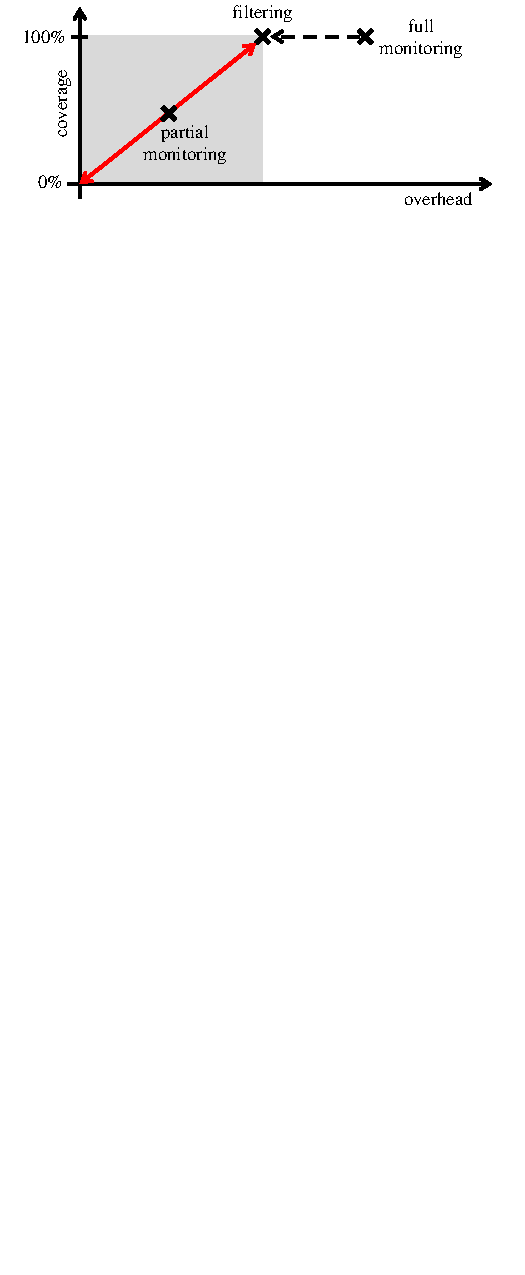
\includegraphics[width=\columnwidth]{figs/optimization_overview.pdf}
    \vspace{-0.2in}
    \caption{Filtering can be used to reduce the overheads. Partial monitoring
    allows a further trade-off between coverage and overheads.}
    \label{fig:optimizations.overview}
    \vspace{-0.1in}
  \end{center}
\end{figure}

The overheads of monitoring can be high. Figure~\ref{dummy} shows the full
monitoring overheads for three example monitoring extensions: array bounds
check (BC), uninitialized memory check (UMC), and dynamic information flow
tracking (DIFT). In order to reduce these overheads, we present two
optimizations. The first is to filter out monitoring events which relate to
null metadata (Section~\ref{sec:optimizations.filter}). Second, in order to
further reduce overheads, we propose to trade-off monitoring coverage. By
performing partial monitoring, we can further decrease the overheads incurred
due to monitoring. Figure~\ref{fig:optimizations.overview} shows an overview of
these ideas. Filtering allows us to reduce the overheads of monitoring and
partial monitoring allows us to further reduce overheads and create a trade-off
between overheads and coverage.

\subsection{Filtering Null Metadata Events}
\label{sec:optimizations.filter}

The instruction-grained run-time monitoring schemes we focus on typically set
and keep track of metadata information. This metadata information is used to
verify security or reliability probabilities. For example, for array bounds
check, the monitoring core stores metadata describing the base and bounds
addresses for array pointers. This metadata is checked on load and store
instructions. If the metadata for an event is null, then it is not relevant to
array bounds check since this represents a non-array pointer object. By
filtering out these null monitoring events, we can reduce the overheads of
monitoring by reducing the amount of work the monitoring core must do.

In order to filter out null monitoring events, we need an efficient method to
keep track of which events are null. In addition, when we filter out a null
monitoring event, we must ensure that any metadata updates that were skipped
are handled properly. Typically, these null monitoring events are just
propagating this null metadata information. Thus, when we filter out one of
these events, we must ensure that the destination operand is marked as null. In
other words, we need to be able to track the dataflow for these null metadata.

\subsection{Trading-Off Coverage for Reduced Overheads}
\label{sec:optimizations.drop}

There is a limit to the reduction in overheads by using filtering. We propose
that overheads can be further reduced by performing partial monitoring. As the
monitoring schemes we target consist of a large number of independent
monitoring checks, it can still be possible to provide partial protection by
performing a portion of the monitoring operations. Thus, we aim to enable this
trade-off between overheads and monitoring coverage.

The high-level idea is to track the run-time monitoring overheads. When the
overhead exceeds our target overhead, we will drop monitoring operations.  Of
course, dropping monitoring operations implies that some functionality of the
monitoring scheme has been lost.  This may cause either false negatives, where
an error that occurs in the main program's execution is not detected, or false
positives, where the monitor incorrectly believes an error has occurred.  For
example, a false positive can occur for array bounds check if an event is
dropped that handles copying a pointer. A subsequent array access using the new
pointer will incorrectly cause an error to be raised since the new pointer's
base and bounds will not be correctly set.  We accept false negatives as the
loss in coverage that we trade off in order to limit overheads.  However, we
must safely drop monitoring events in such a way as to avoid false positives so
that the system does not incorrectly raise an error.

In analyzing various monitoring schemes, we found that monitoring operations
are primarily of two types: \emph{checks} and \emph{metadata updates}. Monitors
\emph{check} certain properties to ensure correct main program execution and
they \emph{update} metadata for bookkeeping. Skipping a check operation can
only cause false negatives and will never cause a false positive. Therefore, we
may simply skip a check operation. Skipping an update operation can cause false
negatives but may also cause false positives. Essentially, when an update
operation is skipped, we can no longer trust the corresponding metadata. Thus,
we need to be able to mark these invalid metadata. Furthermore, metadata that
would be derived from these dropped events also will be invalid. In other
words, we need to be able to track the dataflow of invalid metadata when
monitoring operations are dropped.

\section{Monitoring Architecture Model}
\label{sec:arch}

% Run-time monitoring overview
\begin{figure}
  \begin{center}
    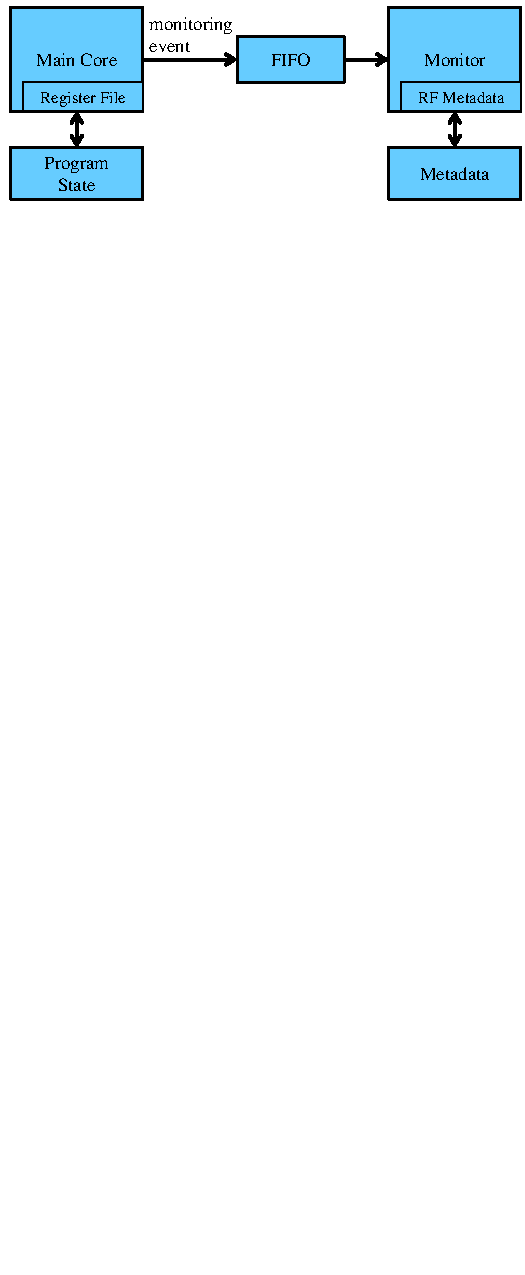
\includegraphics[width=\columnwidth]{figs/monitoring_architecture.pdf}
    \vspace{-0.2in}
    \caption{Overview of run-time monitoring architecture.}
    \label{fig:arch.overview} 
    \vspace{-0.2in}
  \end{center}
\end{figure}

Figure~\ref{fig:arch.overview} shows an overview of the run-time monitoring
model that is assumed in this paper. 
% The \emph{main task} is a computation task that performs the original function
% of the real-time system and is run on the \emph{main core}. 
The \emph{main program} is a computation task that performs the original
function of the system and is run on the \emph{main core}.
% The main task has a
% worst-case execution time (WCET) which can be upper-bounded using a variety
% of existing techniques \cite{wcetsurvey-tecs08}. This WCET is used for timing
% analysis in the design of the real-time system. As long as the execution
% time of the main task does not exceed this bound, then all timing guarantees
% from the analysis hold.
On certain events
during the main program, such as the execution of certain types of
instructions, the \emph{monitor} performs a series of \emph{monitoring
operations}. The monitor operates in parallel to the main core. These events
are referred to as
\emph{monitoring events}. Depending on the type of a monitoring event, different
monitoring operations are executed. Monitoring events are buffered
in a FIFO
structure to decouple the running of the main core and the monitor. If the FIFO
is full, then the main core is forced to stall on a monitoring event until a
FIFO entry becomes available. For programmable monitors, these stalls are a
major source of overhead because the monitor may take several cycles to process
a single event from the main core. We refer to these stalls and other
overheads,
such as contention for shared resources, as
\emph{monitoring overheads}. If the monitor detects an %inconsistent or
undesired behavior in the monitoring events, then an error is detected. 
% We do
% not focus here on the question on how to handle such an error. However, there are
% several options on how to handle an error such as raising an exception,
% notifying the user, or switching to a simpler, more trusted main task
% \cite{sha-simplex-sw01}.

There are many possible monitoring schemes that can be implemented on this
type of fine-grained parallel monitoring architecture such as
array bound checks \cite{devietti-hardbound-asplos08}, memory protection \cite{mmp02}, 
information flow tracking \cite{suh-dift-asplos04, greathouse-testudo-micro08}, 
soft error detection \cite{argus-micro07}, data-race detection \cite{cord-hpca06}, etc.
One example is an
uninitialized memory check (UMC) where 
monitoring is used to detect when software attempts to read from a memory location that
was not previously initialized. This can be done by forwarding each load and store
instruction from the main core to the monitor.
%the memory address
%of each store and load instruction on the main core to the monitor as
%well as whether the instruction was a store or load. 
For every memory location,
the monitor keeps one bit of metadata. On a store to a
memory location, the monitor marks the corresponding metadata bit to
indicate that the memory location has been initialized. On a load,
the monitor checks that the corresponding metadata bit has
been previously marked as initialized.

There are multiple options for implementing programmable parallel monitors. For example, the
Log-Based Architecture \cite{chen08-lba} uses processor cores in a multi-core
system as monitors. The FlexCore architecture \cite{deng-flexcore-micro10}
instead uses an FPGA-fabric to implement the monitor. The approach we describe
in this paper applies to any of these parallel monitors. However, for experiments,
we model an FPGA-based monitor similar to FlexCore. 
%Specifically, this
%architecture uses an on-chip FPGA fabric to
%allow high-performance and reconfigurable run-time monitoring. 
The on-chip FPGA fabric is
used to implement the ``Monitor'' block in Figure~\ref{fig:arch.overview}
while the FIFO from the main core and metadata cache are implemented as ASICs.

\section{Dropping Policies}
\label{sec:policies}

In order to use partial monitoring to enable adjustable overheads, we must also
specify a policy for when and which monitoring events are dropped. In this
section, we discuss some of the options and trade-offs for dropping policies.
We split this decision into two components:
\begin{enumerate}
  \item When do we need to drop events in order to enable reduced overheads? (Section~\ref{sec:policies.when})
  \item Which events should be dropped? (Section~\ref{sec:policies.which})
\end{enumerate}

% Our goal with enabling partial monitoring is to allow for a specified overhead target or budget to be met while maximizing the amount of monitoring performed.
% This is done by dynamically dropping a portion of the monitoring operations. In this section, we discuss in detail how this dropping decision is
% made. Specifically, we first discuss how to decide when dropping should be performed 
% Section~\ref{sec:policies.slack}. Next, we investigate trade-offs created by
% selecting which events are dropped (Section~\ref{sec:policies.events}). Different policies in determining which
% events can be dropped create a trade-off between how closely the overhead
% budget is met and the monitoring coverage achieved.

\subsection{Deciding When to Drop}
\label{sec:policies.when}

% Slack
\begin{figure}
  \begin{center}
    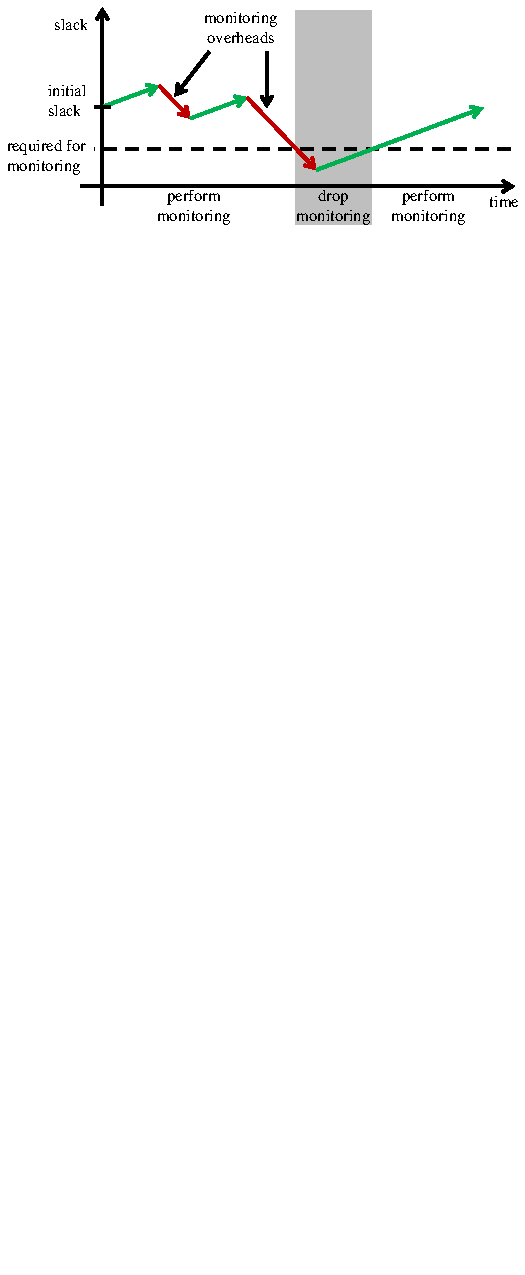
\includegraphics[width=\columnwidth]{figs/slack.pdf}
    \vspace{-0.3in}
    \caption{Slack and its effect on monitoring over time.}
    \label{fig:policies.slack}
    \vspace{-0.1in}
  \end{center}
\end{figure}

In this section, we discuss two possible ways to determine when events should be dropped.
The first possibility is to probabilistically drop events. By setting the probability of
dropping events appropriately, overheads can be reduced. This works well for
enabling partial monitoring for cooperative testing and debugging since the
randomness allows different users and runs to monitor different portions of the
program. However, using a probabilistic dropping policy can make it difficult
to meet a target overhead without prior profiling.

Alternatively, we can specify a target overhead and estimate, at run-time, the
overheads of monitoring in order to decide whether dropping is needed.
The overhead budget is specified as a percentage of the main program's execution
cycles without monitoring. We define \emph{slack} as the number of cycles of
monitoring overhead that can be incurred while staying within the budget
target. Slack is essentially the difference between the actual overheads seen
and the budget specified. Slack is generated as the main program runs and consumed as monitoring overheads occur.  For
example, if no monitoring overheads occur during 1000 cycles of the main
program's execution and the designer sets a 20\% overhead target, then the
slack that is built up during this period is 200 cycles. If the main core is
then stalled for 50 cycles due to monitoring, then the remaining slack is 150
cycles. 
In addition to this accumulated slack, a small amount of initial slack
can be given in order for monitoring to be performed at the start of a program.
Figure~\ref{fig:policies.slack} shows an example of how slack can change over time.
In this slack-based policy, if the slack falls below zero (i.e., the overhead budget is exceeded), then
monitoring events should be dropped.

% % Slack tracking module
% \begin{figure}
%   \begin{center}
%     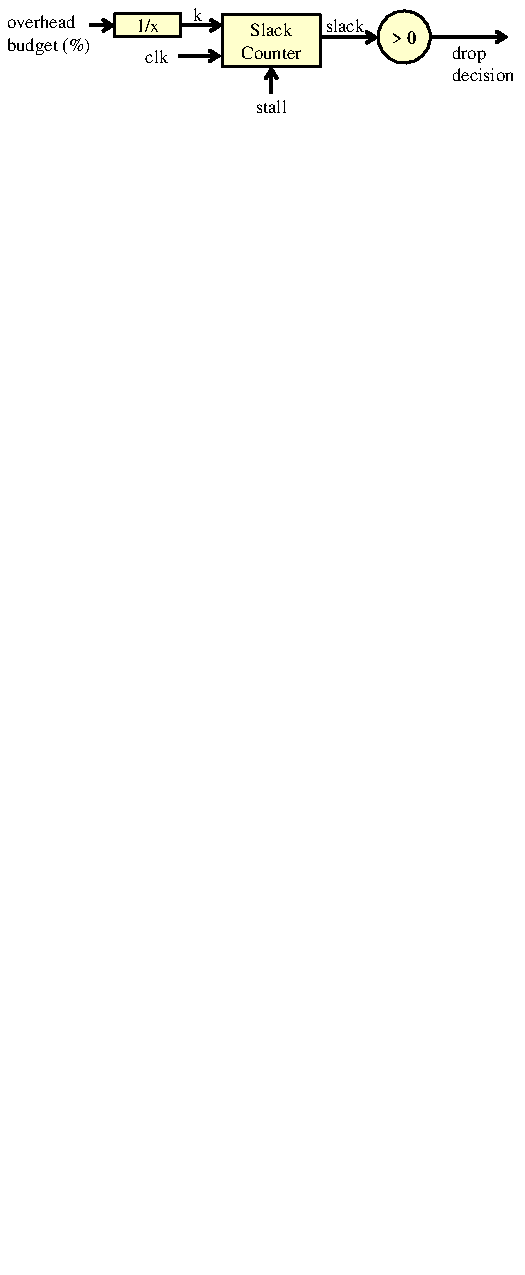
\includegraphics[width=\columnwidth]{figs/stm.pdf}
%     \vspace{-0.2in}
%     \caption{Slack tracking and drop decision hardware.}
%     \label{fig:policies.stm}
%     \vspace{-0.1in}
%   \end{center}
% \end{figure}

% Figure~\ref{fig:policies.stm} shows a hardware slack tracking module for
% keeping track of slack. 
Slack can be easily measured in hardware by using a counter that increments on every $k$-th
cycle of the main core (e.g., every 5th cycle for a 20\% target budget). 
% This $k$ can be calculated by taking the reciprocal of
% the target budget. For example, if the target budget is 20\%, then the counter
% increments on every 5th clock cycle. 
The value of this counter is the
accumulated slack. Whenever the main core is stalled due to the monitor, the
measured slack is decremented. It is difficult to precisely determine the
entire impact of monitoring on the main core due to the
difficulty in measuring certain overheads such as contention for shared memory.
However, we have found that using only the stalls due to FIFO back pressure
works well in practice.

\subsection{Deciding Which Events to Drop} 
\label{sec:policies.which}

% % Varying slack's impact on coverage for UMC
% \begin{figure}
%   \begin{center}
%     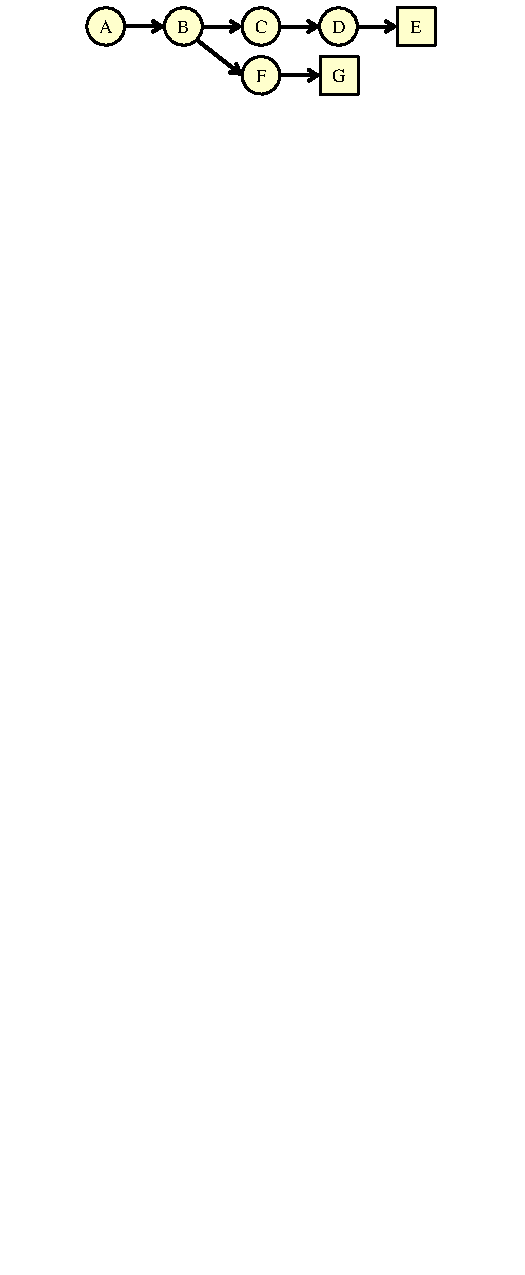
\includegraphics[width=\columnwidth]{figs/dataflow_graph.pdf}
%     \vspace{-0.3in}
%     \caption{Example dependence graph for metadata. Square nodes represent
%     events where checks are performed.} 
%     \label{fig:policies.dataflow_graph}
%     \vspace{-0.1in}
%   \end{center}
% \end{figure}

\begin{figure}
  \begin{center}
  \subfloat[unrestricted dropping]{
    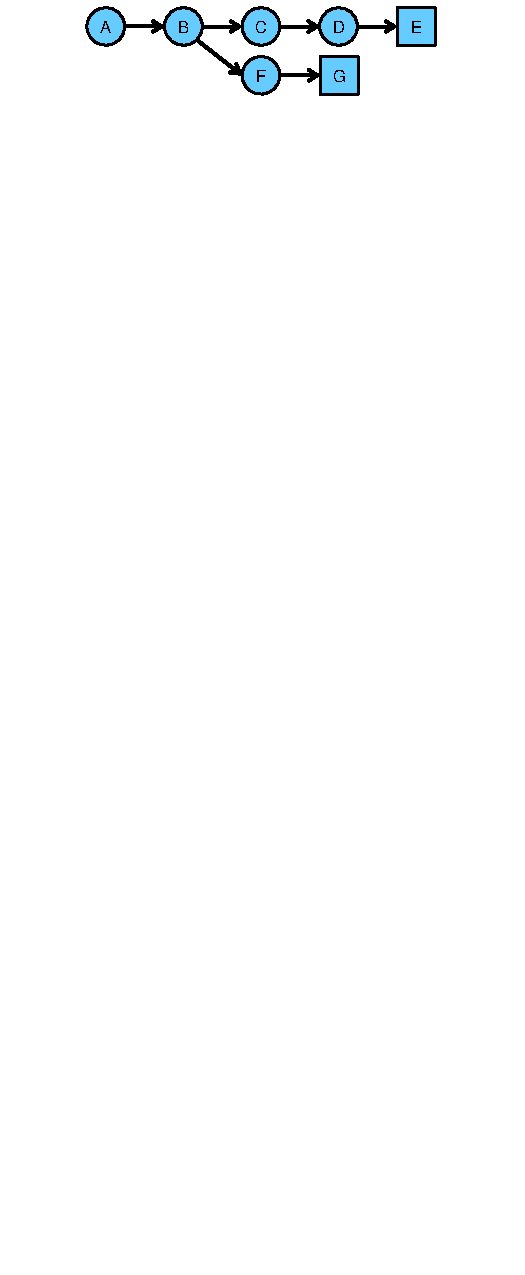
\includegraphics[width=\columnwidth]{figs/all_drop.pdf}
    \label{fig:policies.all_drop}
  }
  \vspace{-0.1in}
  \\
  \subfloat[source-only dropping]{
    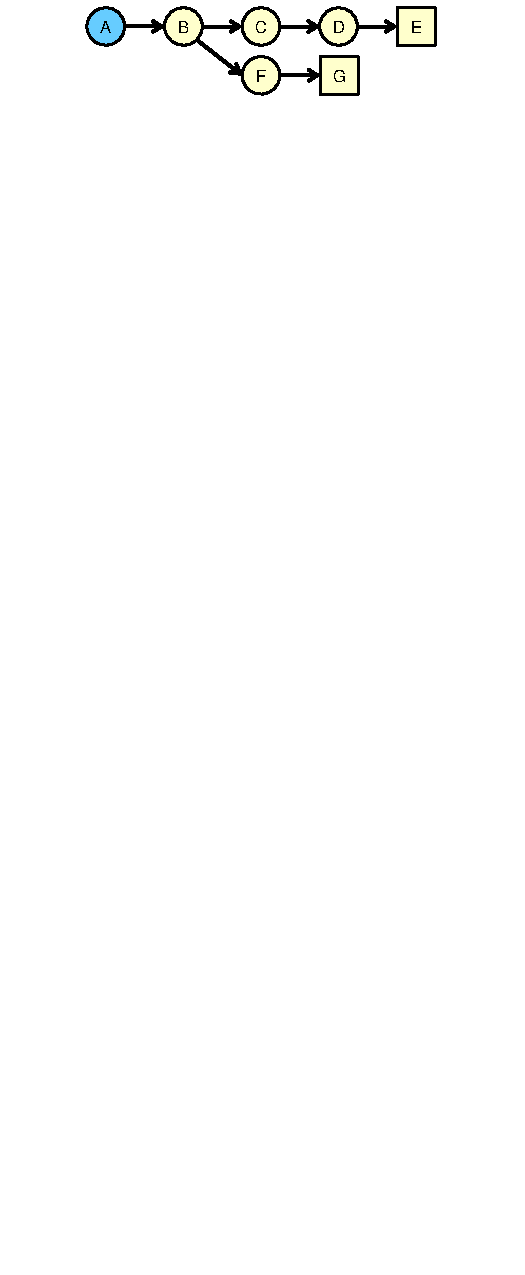
\includegraphics[width=\columnwidth]{figs/source_drop.pdf}
    \label{fig:policies.source_drop}
  }
  \vspace{-0.1in}
%   \\
%   \subfloat[sub-flow dropping]{
%     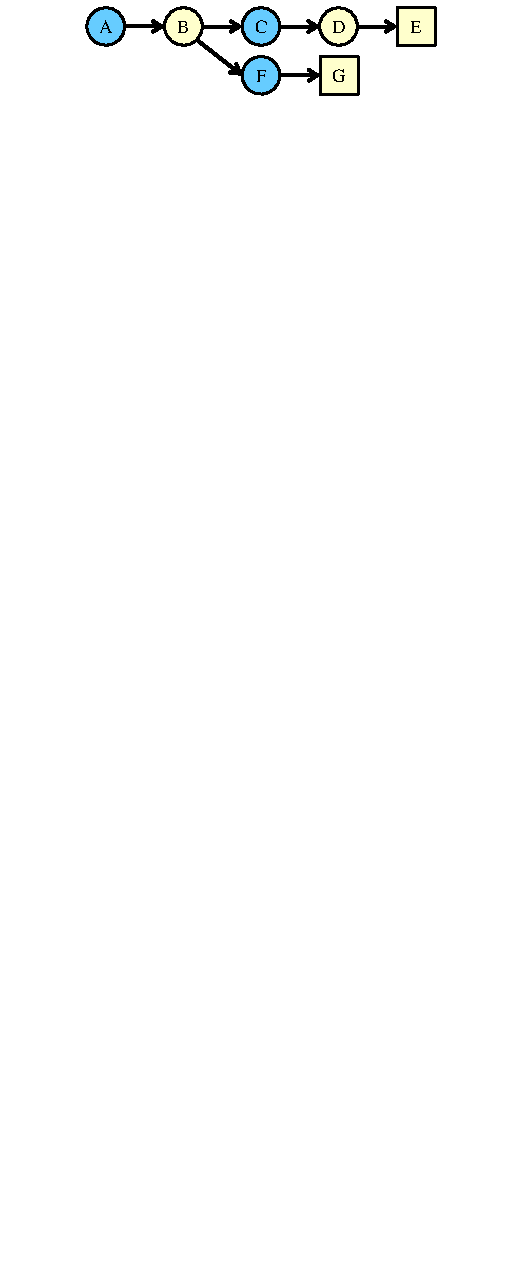
\includegraphics[width=\columnwidth]{figs/min_drop.pdf}
%     \label{fig:policies.min_drop}
%   }
  \end{center}
  \vspace{-0.1in}
  \caption{Comparison of dropping policies using metadata dependence graphs.
  Square nodes represent events where check are performed. Blue (dark) nodes
  indicate which nodes can be dropped.}
  \label{fig:policies.policies}
\end{figure}

In addition to deciding when dropping is required, trade-offs also exist in
deciding which events should be dropped.
The simplest policy is to drop any monitoring events when slack is less than or equal to zero.  However, this can result in
wasted work. For example, consider the metadata dependence graph shown in
Figure~\ref{fig:policies.all_drop}. Here, an edge from node {\tt A} to node
{\tt B} represents that if event {\tt A} is dropped, then due to its
invalidated metadata, it will cause event {\tt B} to be dropped. Square
nodes indicate events where monitoring checks are performed. In the
example, suppose that event {\tt E} is meant to perform a check operation but is dropped.
In this situation, the
monitoring operations that were done for events {\tt C} and {\tt D} were wasted
since their results were not used for any monitoring checks.
That is, by the time we decide to drop event {\tt E}, we have already 
updated metadata due to events {\tt C} and {\tt D} which is no longer needed.

An alternative dropping policy which eliminates this wasted work is to only make dropping decisions at
the root of these metadata flows. That is, we will decide to either monitor or
not monitor an entire metadata flow. We refer to this dropping decision policy
as \emph{source-only dropping} and we refer to the previous policy of 
dropping any event as \emph{unrestricted dropping}.

Figures~\ref{fig:policies.all_drop} and \ref{fig:policies.source_drop} show a
comparison of where dropping decisions are made for these two policies. Source
dropping will
result in no wasted work and thus better coverage. However, because of the coarser-grained decision, it
may be more difficult to closely match overheads. We expect source-only dropping 
to work well when there are a large number of independent metadata flows.
In addition, using a probabilistic dropping policy works poorly with
unrestricted dropping. Since each event in a dependent chain (e.g., events {\tt
A} through {\tt E}) needs to be monitored in order for the monitoring check to
be useful, randomly dropping any single event will cause the final check to be
invalid.

Depending on the target application of partial monitoring, different policies
are more applicable.
For applications where closely matching an overhead target is important, a
slack-based, unrestricted dropping policy is appropriate. However, if matching
the overhead target is not as important, then a slack-based, source-only dropping
policy could provide better coverage. 
Finally, if the goal is to use partial monitoring to enable cooperative
debugging and testing with very low overheads, then a probabilistic,
source-only dropping policy can be used to provide good total coverage over
multiple runs.

% Trade-off between source-drop and unrestricted dropping
% \begin{figure}
%   \begin{center}
%     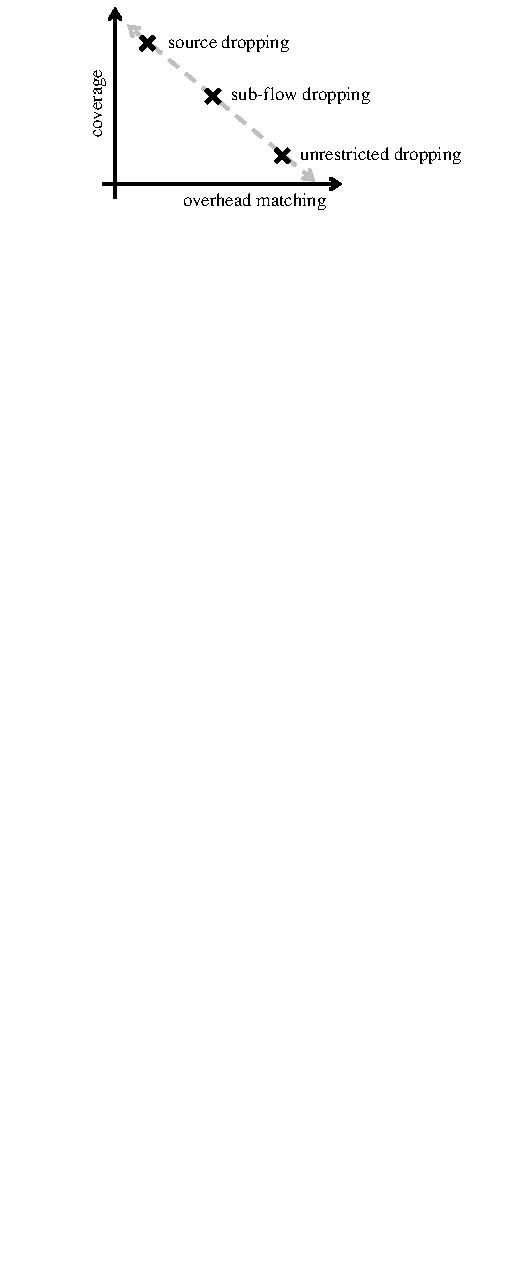
\includegraphics[width=\columnwidth]{figs/policy_trade_off.pdf}
%     \vspace{-0.3in}
%     \caption{Slack tracking and drop decision hardware.}
%     \label{fig:policies.trade_off}
%     \vspace{-0.2in}
%   \end{center}
% \end{figure}
% 
% Another possible method is to make the dropping decisions somewhere in between
% source-only dropping and unrestricted dropping. From the graph in 
% Figure~\ref{fig:policies.dataflow_graph}, we can see that if the dropping
% decision is made at event {\tt C} then we can skip event {\tt E} with no wasted
% work. If we instead choose to perform monitoring for event {\tt C}, then we want to perform all
% monitoring on that flow. Similarly, event {\tt F} creates a decision point for
% the bottom flow that will result in no wasted work and dropping event {\tt A}
% allows the entire shown metadata flow to be dropped with no wasted work. If the
% program can be
% analyzed or profiled to identify these instructions which, if dropped, lead to
% no wasted work, then this information can be used at run-time to minimize the
% amount of wasted work. We refer to this policy as \emph{sub-flow dropping}.
% Figure~\ref{fig:policies.min_drop} shows the points were dropping decisions are
% made for this policy.
% Sub-flow dropping is a coarser-grained decision than unrestricted dropping, but
% finer-grained that source-only dropping. Thus, its ability to match overheads is
% expected to sit between these other two policies. Similarly, there still exists
% edge cases where wasted work can occur, but typically we expect much less
% wasted work than unrestricted 
% dropping. Thus, we expect the coverage achieved by sub-flow dropping for a
% certain overhead to fall between source-only and unrestricted dropping. These three
% dropping policies create a trade-off space between coverage achieved and
% ability to match an overhead target.
% Figure~\ref{fig:policies.trade_off} summarizes this trade-off between coverage
% and ability to match overhead.


% \section{Reducing Monitoring Overheads}
\label{sec:filter}

The instruction-grained monitoring techniques we consider forward all
instructions of certain types (e.g., load instructions) to the monitoring core.
However, not all of these forwarded instructions have relevant monitoring to be
done. For example, for array bounds check, all load and store instructions are
forwarded. However, only loads and stores associated with array pointers have
relevant checking to be done. Thus, we could greatly reduce the amount of
monitoring done by only forwarding instructions that correspond to data that
correspond to array pointers and have been marked with base and bound metadata.
More generally, we can reduce monitoring overheads by filtering out certain
events that correspond to empty (i.e., uninitialized) metadata.

% Overview of inserting dataflow engine
\begin{figure}
  \begin{center}
    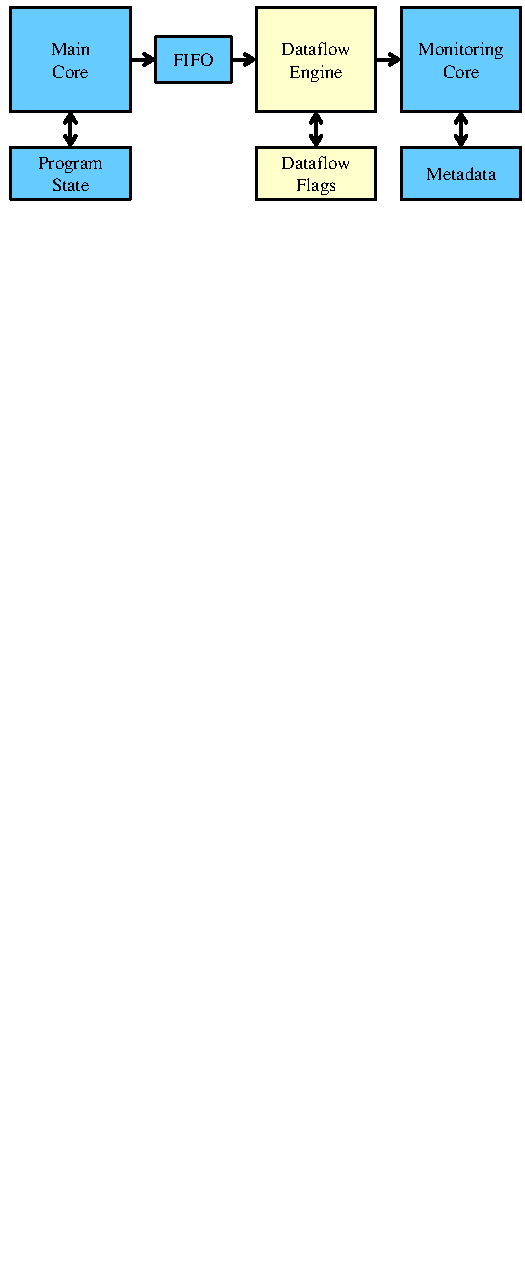
\includegraphics[width=\columnwidth]{figs/dataflow_overview.pdf}
    \vspace{-0.2in}
    \caption{The dataflow engine is inserted between the main core and the monitoring core.}
    \label{fig:filter.overview} 
    \vspace{-0.1in}
  \end{center}
\end{figure}

In this section, we describe how a DIFT-like hardware engine can be used to track
whether metadata has been initialized. We use this information to filter out
monitoring operations for uninitialized metadata. This engine sits between the
main core and the monitoring core (see Figure~\ref{fig:filter.overview}).

\subsection{Initialized Metadata}

% Detailed architecture of dataflow engine
\begin{figure*}
  \begin{center}
    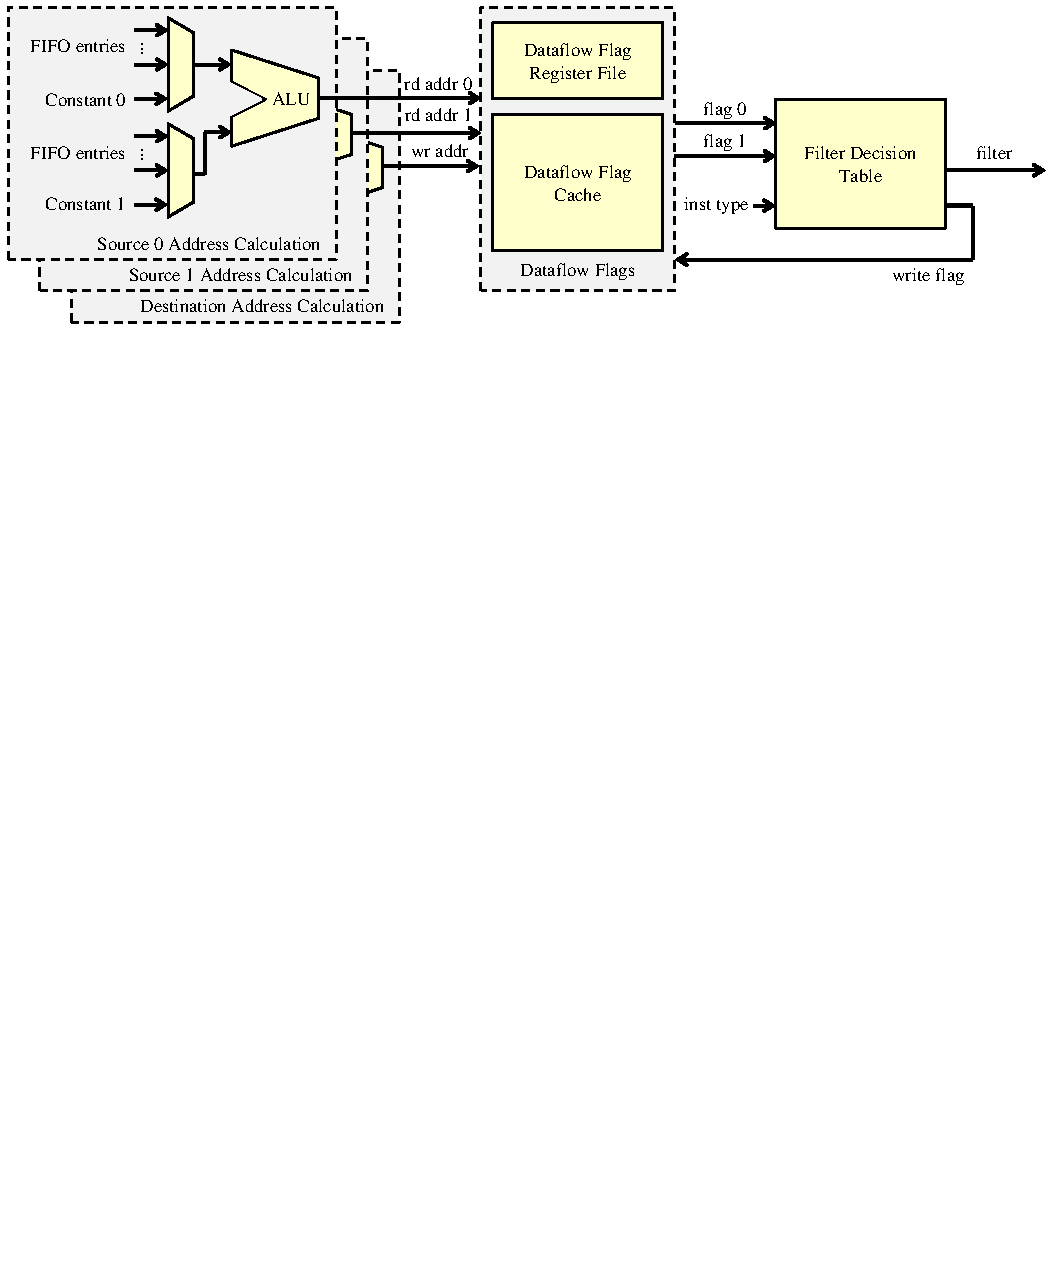
\includegraphics[width=\linewidth]{figs/dataflow_architecture.pdf}
    \vspace{-0.3in}
    \caption{Hardware architecture of dataflow engine.}
    \label{fig:filter.architecture} 
    \vspace{-0.1in}
  \end{center}
\end{figure*}

Figure~\ref{fig:filter.architecture} shows a block diagram of the hardware for keeping track of
initialized metadata. When metadata is initialized, the monitor sends a signal
to the DIFT engine to mark a corresponding initialization flag. Similarly, when
the monitor propagates metadata, it also sends a signal to initialize the
metadata that has been written to. When a new event arrives at the DIFT engine,
it will read in up to two initialization flags. A table is used to configure
which initialization flags should be read in depending on the instruction type of
the event and information from the monitoring event. A pair of simple ALUs is
used to allow calculating memory addresses based on information from the
monitoring event. Typically, the initialization flags read correspond to the
source operands of the monitored instruction.

Given this set of initialization flags, a Filter Decision Table decides, based
on instruction type, whether an event can be filtered out. This table is
configured based on the specific semantics of a monitoring technique.
Typically, if all initialization flags are marked as uninitialized, then the
event can be filtered out. For example, for array bounds check, if the source
register's metadata is marked as uninitialized, then this means that the
register does not correspond to an array pointer. Thus, we can filter out
performing monitoring for this event.

\subsection{Propagating Initialization Flags}

If the source operands are marked as uninitialized, then typically we can
filter out this event. However, in these cases, the monitor also typically
resets the destination operand's metadata as cleared or uninitialized.
Thus, when we filter out one of these events, we need to also propagate the
uninitialized flag to the destination. The Filter Decision Table includes this
information about whether the destination operand metadata should be marked as
uninitialized.

% 
% Operation of hardware modules

\begin{tabular}{|l|l|l|l|}
\hline

{\bf Monitor} & {\bf Event} & {\bf Filter Condition} & {\bf Dropping/Filter Operation} \\ \hline \hline

\multirow{4}{*}{BC}  
& Array allocation & Never & Invalidate array pointer \\ \cline{2-4}
& ALU   & At least one invalid source register & Invalidate destination register \\ \cline{2-4}
& Load  & Invalid source memory location & Invalidate destination register \\ \cline{2-4}
& Store & Invalid source register & Invalidate destination memory location \\
\hline\hline

\multirow{2}{*}{UMC}  
& Store & Never & Invalidate destination memory location \\ \cline{2-4}
& Load & Invalid source memory location & Do nothing \\ 
\hline\hline

\multirow{5}{*}{DIFT}  
& Software set tag & Never & Invalidate destination memory location \\ \cline{2-4}
& ALU   & At least one invalid source register & Invalidate destination register \\ \cline{2-4}
& Load  & Invalid source memory location & Invalidate destination register \\ \cline{2-4}
& Store & Invalid source register & Invalidate destination memory location \\ \cline{2-4}
& Indirect jump & Invalid source metadata & Do nothing \\ 
\hline


\end{tabular}

% \section{Application to Monitoring Schemes}
\label{sec:extensions}

% Monitoring operations
\begin{table*}[tb]
  \begin{center}
    \begin{small}
    
% Summary of monitoring operations

\begin{tabular}{|l|l|l|}
\hline

{\bf Monitor} & {\bf Event} & {\bf Monitoring Operation} \\ \hline \hline

\multirow{4}{*}{BC}  
 & Array allocation & Set base and bound metadata \\ \cline{2-3}
 & ALU & Copy metadata from register to register \\  \cline{2-3}
 & Load & Copy metadata from memory to register. Check memory access address. \\ \cline{2-3}
 & Store & Copy metadata from register to memory. Check memory access address. \\ 
\hline\hline

\multirow{2}{*}{UMC}  
 & Store & Set metadata tag (data initialized) \\ \cline{2-3}
 & Load & Check if metadata tag is set \\ 
\hline\hline
% & Software clear tag & Clear metadata tag & Non-critical \\ \hline\hline

\multirow{5}{*}{DIFT}  
 & Software set tag & Set tag to a specified identifier value based on software command \\ \cline{2-3}
 & ALU & If input tags are different, output tag is a new identifier. Otherwise, output tag is the input tag. \\ \cline{2-3}
 & Load & Set register tag as tag of loaded data \\ \cline{2-3}
 & Store & Set memory tag as register tag \\ \cline{2-3}
% & Software clear tag & Clear tag & Update \\ \cline{2-4}
 & Indirect jump & Check tag \\ 
 \hline

% \multirow{5}{*}{BC}  
%  & MOV/LD/ST          & Propagate colors (Tag[dest] = Tag[src]) & Critical \\ \cline{2-4}
%  & ADD/SUB/NOT        & Update colors (Tag[dest] = f(Tag[src])) & Critical \\ \cline{2-4}
%  & OR/XOR             & Clear colors & Critical \\ \cline{2-4}
%  & LD/ST              & Compare pointer and memory colors & Check \\ \cline{2-4}
%  & Software set color & Set pointer colors & Critical \\ \hline\hline

% Soft Error Check & Instruction & Check instruction computation & Check \\ \hline\hline
% 
% \multirow{2}{*}{Bank of Observers}  
%  & System output & Update state estimation & Critical \\ \cline{2-4}
%  & New state estimate & Check that states of all observers matches & Check \\ \hline

\end{tabular}

    \end{small}
    \caption{Monitoring operations for BC, UMC, and DIFT.}
    \label{tab:extensions.monitor}
    \vspace{-0.2in}
  \end{center}
\end{table*}

% Filtering operations for clean flags
\begin{table*}[tb]
  \begin{center}
    \begin{small}
    
% Operations for handling clean flags

\begin{tabular}{|l|l|l|l|}
\hline

{\bf Monitor} & {\bf Event} & {\bf Filter Condition} & {\bf Filter Operation} \\ \hline \hline

\multirow{4}{*}{BC}  
& Array allocation & Never & - \\ \cline{2-4}
& ALU   & Both source registers are clean & Mark destination register as clean \\ \cline{2-4}
& Load  & Source memory location is clean & Mark destination register as clean \\ \cline{2-4}
& Store & Source register is clean & Mark destination memory location as clean \\
\hline\hline

\multirow{2}{*}{UMC}  
& Store & Never & - \\ \cline{2-4}
& Load & Source memory location is dirty & Do nothing \\ 
\hline\hline

\multirow{5}{*}{DIFT}  
& Software set tag & Never & - \\ \cline{2-4}
& ALU   & Both source registers are clean & Mark destination register as clean \\ \cline{2-4}
& Load  & Source memory location is clean & Mark destination register as clean \\ \cline{2-4}
& Store & Source register is clean & Mark destination memory location as clean \\ \cline{2-4}
& Indirect jump & Source register is clean & Do nothing \\ 
\hline


\end{tabular}

    \end{small}
    \caption{Filtering conditions and operations for clean flags.}
    \label{tab:extensions.filter}
    \vspace{-0.2in}
  \end{center}
\end{table*}

% Filtering operations for invalid flags
\begin{table*}[tb]
  \begin{center}
    \begin{small}
    
% Operation of hardware modules

\begin{tabular}{|l|l|l|l|}
\hline

{\bf Monitor} & {\bf Event} & {\bf Filter Condition} & {\bf Dropping/Filter Operation} \\ \hline \hline

\multirow{4}{*}{BC}  
& Array allocation & Never & Invalidate array pointer \\ \cline{2-4}
& ALU   & At least one invalid source register & Invalidate destination register \\ \cline{2-4}
& Load  & Invalid source memory location & Invalidate destination register \\ \cline{2-4}
& Store & Invalid source register & Invalidate destination memory location \\
\hline\hline

\multirow{2}{*}{UMC}  
& Store & Never & Invalidate destination memory location \\ \cline{2-4}
& Load & Invalid source memory location & Do nothing \\ 
\hline\hline

\multirow{5}{*}{DIFT}  
& Software set tag & Never & Invalidate destination memory location \\ \cline{2-4}
& ALU   & At least one invalid source register & Invalidate destination register \\ \cline{2-4}
& Load  & Invalid source memory location & Invalidate destination register \\ \cline{2-4}
& Store & Invalid source register & Invalidate destination memory location \\ \cline{2-4}
& Indirect jump & Invalid source metadata & Do nothing \\ 
\hline


\end{tabular}

    \end{small}
    \caption{Filtering conditions and operations performed for a dropped or filtered event for invalid flags.}
    \label{tab:extensions.drop}
    \vspace{-0.2in}
  \end{center}
\end{table*}

In this section, we show examples of how our architecture can be applied to
three specific monitoring schemes: array bounds check (BC), uninitialized
memory check (UMC), and dynamic information flow tracking (DIFT).
Table~\ref{tab:extensions.monitor} shows a summary of the monitoring operations for these
monitoring schemes. Table~\ref{tab:extensions.filter} summarizes when when
monitoring events can be filtered out due to clean metadata and what metadata
needs to be marked as clean on a filtered event.
Table~\ref{tab:extensions.drop} shows the analogous information for the valid
flags. In this case, the operation listed is also the one performed when a
monitoring event is dropped due to insufficient slack. Note that for simplicity
the policies for clean and invalid flags are shown and discussed separately
here. However, the dataflow engine actually operates on pairs of these flags
using a combined policy.

\subsection{Array Bounds Check}

As described in Section~\ref{sec:monitoring}, array bounds check is a
monitoring scheme that attempts to detect buffer overflows where memory
accesses go beyond the boundaries of an array.
Buffer overflows can cause unreliable program execution or create openings for
malicious attackers. One way to detect buffer overflows is a base and bounds
approach \cite{hardbound-asplos08}. In this approach, metadata is
associated with an array pointer when it is allocated that includes the base
(start) address and bound (end) address of the corresponding array. On ALU
instructions, this base and bound metadata is copied to the destination
registers.  On store instructions, the metadata for the source register is
copied to the metadata for the store address. Similarly, on load instructions,
the metadata value for the load address is copied to the destination register's
metadata. In addition, on load and store instructions, the memory address is
checked to be within the base and bounds metadata. If it is not, then an
out-of-bounds error is detected. These operations are summarized in
Table~\ref{tab:extensions.monitor}.

In terms of filtering using clean flags (Table~\ref{tab:extensions.filter}),
array allocations are never filtered since these will always involve non-clean
metadata (i.e., setting new base and bounds). For ALU operations, if both
source operands are clean, then the event can be filtered by setting the
destination register as clean. For load and store, only a single source needs
to be checked to be clean in order for the event to be filtered. Similarly, the
destination register or memory location needs to be marked as clean if the
event is filtered.

The invalid flags for BC operate similarly to the clean flags
(Table~\ref{tab:extensions.drop}). When ALU, load, or store events are dropped or filtered,
the destination register or memory location is marked as invalid. In addition,
we need to handle the possibility of dropping an array allocation. In this
case, the array pointer is marked as invalid. In terms of filtering out invalid
events, for an ALU event, if either of the source registers is invalid then the
event can be filtered. For load and store instructions, if the single source
operand is invalid, then the event can be filtered.

\subsection{Uninitialized Memory Check}

Uninitialized memory check is a monitoring scheme that checks that memory is
written to before it is read from. This is done by forwarding all load and
store instructions to the monitoring core. For every byte of memory, the
monitor keeps one bit of metadata. On a store to a memory location, the monitor
marks the corresponding metadata bit to indicate that the memory location has
been initialized. On a load, the monitor checks that the corresponding metadata
bit has been previously marked as initialized.

Rather than using the clean flags to mirror the initialization metadata that
UMC stores, we use the clean flags as a coarse-grained version of the UMC
metadata in order to more efficiently filter out monitoring operations. We use
a clean flag per word (four bytes) of memory. A clean flag is set to dirty only
if all four of the corresponding memory bytes have been marked as initialized.
On a load, if the clean flag is marked as dirty, then we can filter the event
since we know that all possible corresponding location memory locations have
been marked as initialized. If the flag is marked as clean, then that indicates
that at least one of the corresponding memory bytes has not been initialized
and the monitoring core must perform a further check. Store instructions are
never filtered out.

On a dropped store instruction, the destination memory location is marked as
invalid. On load instructions, we can filter them out if the source memory
location has been invalidated. In this case, we do not have to perform any
further operation since on load instructions since UMC only performs a check
operation for loads.

\subsection{Dynamic Information Flow Tracking}

Dynamic information flow tracking (DIFT) \cite{dift-asplos04} is a security
monitoring scheme that seeks to detect when information from untrusted sources
is used to affect the control flow.  In its simplest form, DIFT keeps a 1-bit
metadata tag for each memory location and each register, indicating tainted or
untainted. When data is read from an untrusted source, it is marked as tainted.
As this data is used for other operations, the results of these operations are
also marked as tainted. On an indirect jump, the taint bit of the register used
is checked. If the register is found to be tainted, then an error is detected.
We focus on a more heavy-weight approach that also tracks some information of
where flows originate from by using a multi-bit (32-bits in our implementation)
metadata tag. This can be used to assist debugging in the case of an error. In
this case, when data is marked from an untrusted source, the software specifies
an identifier to set the metadata tag. This multi-bit tag is propagated on
load, store, and ALU operations. If two different tags are used as sources to
an ALU operation, then a new identifier is calculated based on the sources.
These monitoring operations are summarized in
Table~\ref{tab:extensions.monitor}.

Table~\ref{tab:extensions.filter} shows how the clean flags are used for DIFT.
The rules for ALU, load, and store instructions are same as for array bounds
check. Similar to array allocations, for DIFT, software setting of metadata
tags is never filtered out due to clean metadata. On indirect jump
instructions, if the source register is clean, then the event can be filtered
out as no error has occurred.

Again, the invalid flags for DIFT operate similar to their operation for BC
(Table~\ref{tab:extensions.drop}). In addition to operations for invalidating
destination operands for ALU, load, and store instructions, the destination
memory location is also invalidated when set tag operations dropped. Indirect
jump events are filtered out if the source register is marked as invalid.
However, no further metadata needs to be marked as invalid in this case.

\subsection{Applicability to Other Schemes}

In this section, we have discussed how our dataflow engine can be applied to
three example monitoring schemes to enable reduced and adjustable overheads.
However, our approach can be generally applied to many monitoring schemes. This
is possible because the use of clean and invalidation flags is largely agnostic
to the semantics of the specific monitoring scheme. That is, the dataflow
engine must be configured based on the dataflow of the monitoring scheme, but
it does not need detailed information of what the monitoring scheme does. 

We do note some limitations to the proposed approach. Previous work
\cite{fade-hpca14} that has looked at filtering in order to reduce monitoring
overheads has also filtered out redundant updates where the source metadata
matches the destination metadata. Since we do not read the actual metadata, our
architecture is not able to identify these redundant updates. However, by using
only 2-bit flags, the bandwidth need of our dataflow engine is reduced.  
In addition, we note that filtering using clean flags works well when a large
portion of instructions are not relevant to the monitoring scheme (e.g., array
bounds check only cares about array pointers). However, if most instruction
have dirty metadata, then very little filtering will be possible. 

In terms of using invalidation to perform partial monitoring, this 
approach works best for monitoring schemes where there are many pieces of
independent metadata. Since marking a piece of metadata as invalid will cause
future metadata with dependences to also be marked as invalid, schemes with
large metadata dependency chains can quickly see large amounts of metadata
become invalid. 

Another limitation is that the dataflow engine, as described, only marks one
flag location on each monitoring event. Similarly, the dataflow engine can only
read in two sets of flags in order to determine whether an event can be
filtered or not. This was done because we found that for many monitoring
schemes, the monitoring operations corresponded to program instructions, which
read up to two operands and write to one destination.  For monitoring schemes
which update multiple pieces of metadata on a monitoring event, it may be
adequate to associate a clean and invalid flag with a single piece of metadata.  For
example, a scheme may use a data structure that includes several pieces of
related metadata. On a drop, one of these pieces could be marked as invalid in
order to indicate that the entire structure is invalid.  Similarly, marking one
specified piece as clean may indicate that the entire data structure's metadata
is clean.  Alternatively, the read and write capabilities of the dataflow
engine could be expanded to support more complex monitoring schemes.

\section{Evaluation}
\label{sec:evaluation}

\subsection{Experimental Setup}
\label{sec:evaluation.setup}

We implemented our dataflow-guided monitoring architecture by
modifying the ARM version of the gem5 simulator \cite{gem5} to support parallel
run-time monitoring. We model the main and monitoring cores as running at 2.5
GHz with 4-way set-associative private L1 I/D caches and a shared 8-way 2 MB L2
cache. This setup is similar to the Snapdragon 801 processor commonly found in
mobile systems. The dataflow engine uses a 1 kB cache for flags.

In order to explore the generality of the architecture for
different monitors, we implemented three different monitors: uninitialized
memory check (UMC), array bounds check (BC), and dynamic information flow
tracking (DIFT).  Uninitialized memory check seeks to detect loading from
memory locations that are not initialized first.  Array bounds check, as
mentioned in Section~\ref{sec:monitoring}, is a monitoring scheme that aims to
detect buffer overflows where memory accesses go beyond the boundaries of an
array. We modify the implementation of {\tt malloc} to set base and bound
metadata information. Dynamic information flow tracking is a security
monitoring scheme
which detects when information from untrusted sources is used to affect the
program control flow (i.e., indirect control instructions). For the benchmarks we consider, we mark data read from
files as untrusted. We implemented a multi-bit DIFT scheme which marks
untrusted data with a 32-bit metadata identifier so
that if an error is detected, it is possible to have information about where
the data originated from. 

We tested our system using all C benchmarks from SPECint
CPU2006 \cite{spec2006}. Since our implementation of BC depends on the
modification of {\tt malloc} to set array bounds information, we focus on the C
SPECint benchmarks. Although we do not
show results for the C++ benchmarks, we note that the results for UMC and DIFT
for these benchmarks are similar to the other results shown. For each
benchmark, we simulated for 1 billion instructions. An initial slack of 1
million cycles, which is less than 1\% of
the total execution time, is given for a 10\% target overhead. This initial
slack is scaled proportionally for other overhead targets.

\subsection{Baseline Monitoring Overheads}
% Full monitoring overheads
\begin{figure}
  \begin{center}
    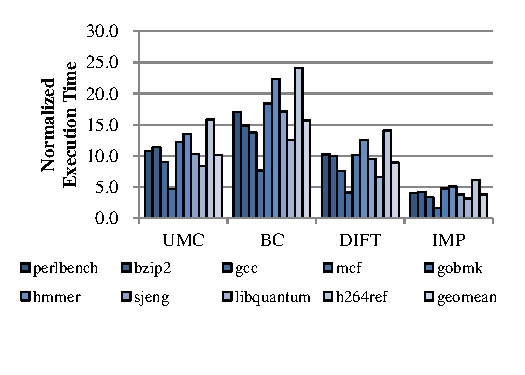
\includegraphics[width=\columnwidth]{figs/data_full_mon.pdf}
    \vspace{-0.2in}
    \caption{Full monitoring overheads for UMC, BC, and DIFT.}
    \label{fig:evaluation.full_mon}
    \vspace{-0.1in}
  \end{center}
\end{figure} Figure~\ref{fig:evaluation.full_mon} shows the execution times of
performing full monitoring normalized to the execution times of the benchmarks
without monitoring. In these results, no filtering or partial monitoring is
done. UMC shows normalized execution times from 4x to 11x with an average
of 7x. BC shows normalized execution times of 9-28x with an average of
18x while DIFT shows normalized execution times of 6x-17x with an average of
11x. One of the reasons for these high overheads is that our implementations of
these monitors dynamically allocate memory for new metadata. This can be an
expensive, many-cycle operation. Statically allocating memory for metadata
will reduce the execution time but requires a large upfront memory footprint
which caused issues with our simulator.

\subsection{Filtering of Monitoring Events}

% Full monitoring overheads
\begin{figure}
  \begin{center}
    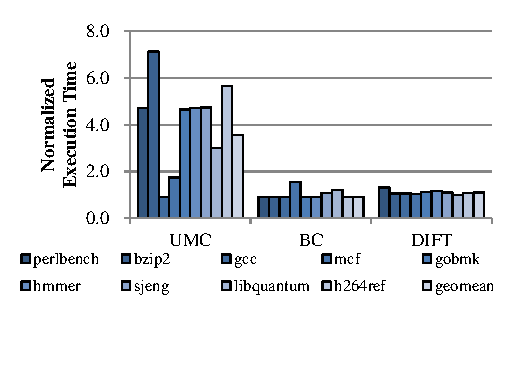
\includegraphics[width=\columnwidth]{figs/data_filtering.pdf}
    \vspace{-0.2in}
    \caption{Monitoring overheads with filtering null metadata for UMC, BC, and DIFT.}
    \label{fig:evaluation.filtering}
    \vspace{-0.1in}
  \end{center}
\end{figure}

Figure~\ref{fig:evaluation.filtering} shows the
normalized execution times with filtering enabled. We see significant
reductions in overhead for all three monitoring schemes. UMC sees normalized
execution times of 2-6x with an average of 4x with null metadata filtering. For BC, normalized execution
times drop from 18x down to 4x on average. The range of normalized execution
times for filtered BC is 1.1-17x. This is not surprising since in the baseline
implementation all loads and stores needed to be monitored. However, with
filtering, only loads and stores corresponding to arrays need to be forwarded.
Finally, DIFT sees the largest reduction in overheads with only 13\% overheads
on average after filtering, with a maximum of 42\%. This is due, in part, to the fact that
for our implementation of DIFT on SPEC
benchmarks, we only mark data read from files as tainted. For most of these
benchmarks, this propagates to relatively few instructions. Instead, if we
targeted network or streaming applications, which have larger amounts of
untrusted input data, we would expect to see less filtering.

\subsection{Coverage with Adjustable Partial Monitoring}

% BC sweep
\begin{figure*}
  \begin{center}
    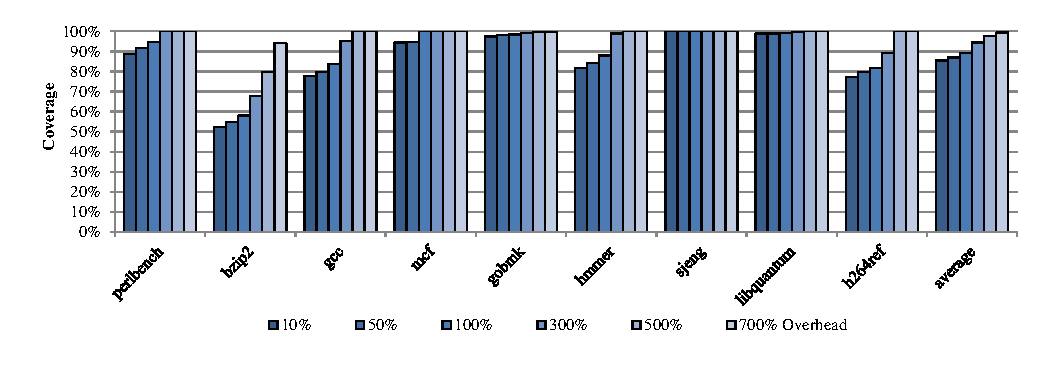
\includegraphics[width=\linewidth]{figs/data_bc_sweep.pdf}
    \vspace{-0.4in}
    \caption{Coverage versus varying overhead budget for array bounds check.}
    \label{fig:evaluation.bc_sweep}
    \vspace{-0.2in}
  \end{center}
\end{figure*}

% UMC sweep
\begin{figure*}
  \begin{center}
    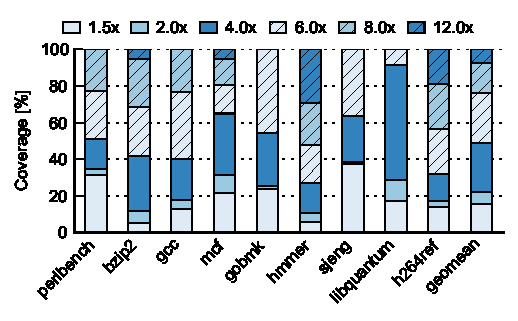
\includegraphics[width=\linewidth]{figs/data_umc_sweep.pdf}
    \vspace{-0.4in}
    \caption{Coverage versus varying overhead budget for uninitialized memory check.}
    \label{fig:evaluation.umc_sweep}
    \vspace{-0.1in}
  \end{center}
\end{figure*}

Although the overheads of DIFT are quite low after filtering, BC and UMC still
show significant overheads. In this section, we evaluate the effectiveness of
using partial monitoring (in addition to filtering) to trade-off coverage for further reduced overheads.
Figure~\ref{fig:evaluation.bc_sweep} shows the monitoring coverage achieved by
array bounds check as we vary the overhead budget. 
We define \emph{monitoring coverage} as the 
percentage of checks that are performed 
(indirect jumps in DIFT, loads in UMC, and memory accesses in BC). 
The metric is chosen to understand
how likely an error/attack instance is to be detected on an individual system. 
While we could not evaluate real errors/attacks due to difficulty in setting up
a large number of bugs and exploits, we believe that the percentage of checks
provides a good estimate of detection probability when errors/attacks are 
uniformly distributed across checks.
Note that this metric is different from the
percentage of monitoring events that are not dropped, which includes
non-check instructions.

We see that by varying the overhead budget, the coverage achieved also varies.
With only a 10\% overhead budget, array bounds check still
achieves 82\% monitoring coverage on average. The high coverage
achieved with such low overheads is due to two main effects.  The first is that
monitoring can be done in parallel, providing monitoring coverage without
introducing overheads. The second effect is that, although we aggressively
filter out monitoring events, there may still exist a large number of
monitoring events that do not lead to security or reliability checks. As a
result, dropping these events can reduce overheads without a large impact on
monitoring coverage.

Figure~\ref{fig:evaluation.umc_sweep} shows the analogous graph for UMC. Again
we see that varying overhead budgets enables partial monitoring. We see that
with a 10\% overhead budget, UMC achieves 32\% monitoring coverage on average.
By increasing this overhead budget to 50\%, UMC achieves 51\% coverage. Even
higher coverage can be achieved by allowing higher overheads.

\subsection{Comparing Dropping Policies}

% UMC exec time
\begin{figure}
  \begin{center}
    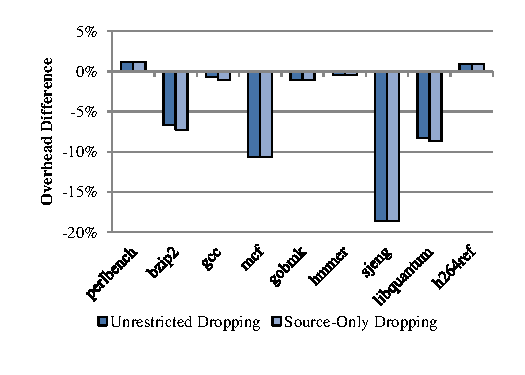
\includegraphics[width=\columnwidth]{figs/data_umc_exec_time.pdf}
    \vspace{-0.2in}
    \caption{Error in meeting overhead budget for uninitialized memory check for different dropping policies.}
    \label{fig:evaluation.umc_exec_time}
    \vspace{-0.2in}
  \end{center}
\end{figure}


% UMC coverage across policies
\begin{figure}
  \begin{center}
    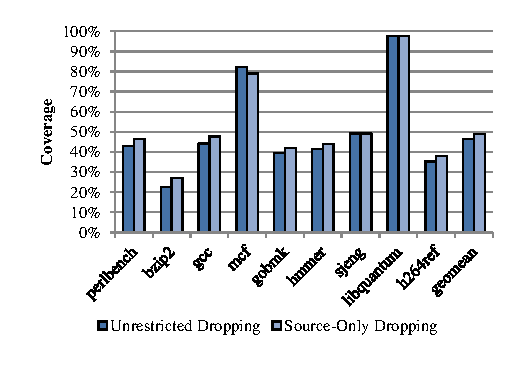
\includegraphics[width=\columnwidth]{figs/data_umc_coverage.pdf}
    \vspace{-0.2in}
    \caption{Coverage for uninitialized memory check for different dropping policies.}
    \label{fig:evaluation.umc_coverage}
    \vspace{-0.1in}
  \end{center}
\end{figure}
In this section we evaluate the trade-offs between unrestricted dropping and source-only dropping.
Figure~\ref{fig:evaluation.umc_exec_time} shows the difference between the
overhead budget and the run-time monitoring overheads for UMC. A positive value
means that the overhead target was overshot while a negative value indicates
that the overhead budget was met. We see similar results for unrestricted
dropping and source-only dropping due to the fact that UMC consists of a large
number of independent monitoring flows.
Figure~\ref{fig:evaluation.umc_coverage} shows the coverage of UMC for
unrestricted dropping and source-only dropping. We see that source-dropping
consistently achieves higher coverage than unrestricted dropping. This is due
to the fact that some of the overheads of monitoring for unrestricted dropping
are being spent on wasted work as discussed in Section~\ref{sec:policies.events}.

% BC exec time
\begin{figure}
  \begin{center}
    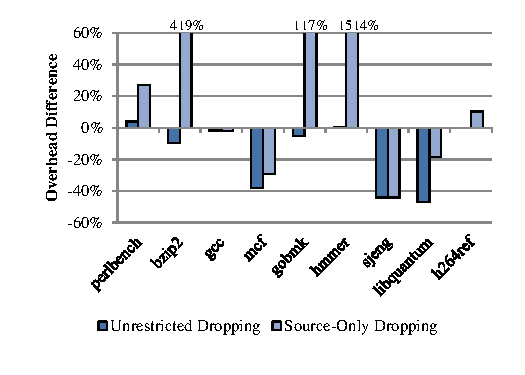
\includegraphics[width=\columnwidth]{figs/data_bc_exec_time.pdf}
    \vspace{-0.2in}
    \caption{Error in meeting overhead budget for array bounds check for different dropping policies.}
    \label{fig:evaluation.bc_exec_time}
    \vspace{-0.2in}
  \end{center}
\end{figure}

% BC coverage across policies
\begin{figure}
  \begin{center}
    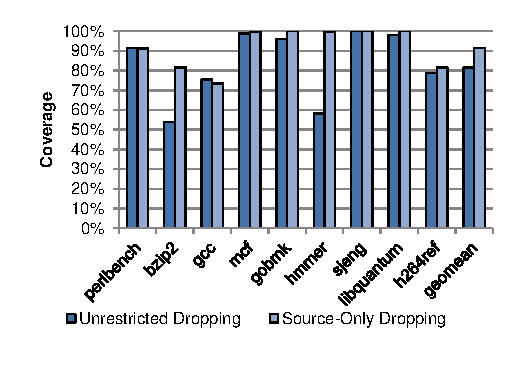
\includegraphics[width=\columnwidth]{figs/data_bc_coverage.pdf}
    \vspace{-0.2in}
    \caption{Coverage for array bounds check for different dropping policies.}
    \label{fig:evaluation.bc_coverage}
    \vspace{-0.2in}
  \end{center}
\end{figure}

Next, we evaluate these trade-offs between source-only dropping and unrestricted dropping for BC.
Figure~\ref{fig:evaluation.bc_exec_time} shows the overhead differences for BC
and Figure~\ref{fig:evaluation.bc_coverage} shows the coverage for BC.
From Figure~\ref{fig:evaluation.bc_exec_time}, we see that for several
benchmarks, source-only drop fails to meet the specified overhead target.
The overshoot of the overhead target is quite high with an overhead difference
of 420\% for {\tt bzip2}, 120\% for {\tt gcc}, and 1500\% for {\tt hmmer}.
Since only array allocations are considered source events for BC, it is
difficult for source-only dropping to match overhead targets. Although
Figure~\ref{fig:evaluation.bc_coverage} again shows higher coverage for
source-only dropping, this is in part due to the fact that is running with
higher overheads.

\subsection{Multiple-Run Coverage}

% Multi-run coverage with unrestricted dropping
\begin{figure}
  \begin{center}
    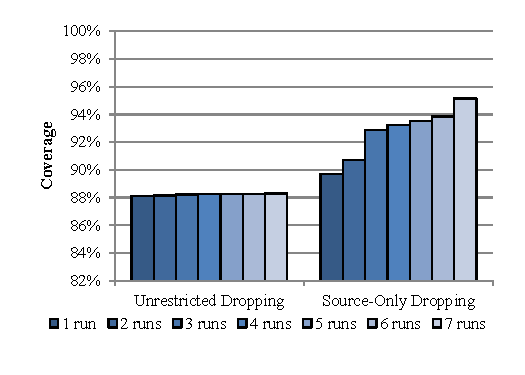
\includegraphics[width=\columnwidth]{figs/data_multirun_coverage.pdf}
    \vspace{-0.2in}
    \caption{Coverage over multiple runs for BC at 10\% overhead with an unrestricted dropping policy.}
    \label{fig:evaluation.multirun}
    \vspace{-0.1in}
  \end{center}
\end{figure}

One possible application of partial monitoring with low overheads is to enable
cooperative debugging. The idea with cooperative debugging is to use partial
monitoring with very low overheads across a large number of users or runs. By
varying the pattern of partial monitoring done on each run, the goal is to
achieve high coverage across multiple runs. Varying the monitoring that is
done for different runs can be achieved by introducing some randomness into the
dropping decision. Figure~\ref{fig:evaluation.multirun} shows the total
coverage achieved over multiple runs for array bounds check running with a 10\%
overhead budget and an unrestricted dropping policy. Each run was simulated for
100 million instructions. For these simulations, events were
dropped probabilistically with the probability scaled proportionally to slack.
That is, when slack is high, the probability of dropping is low and the
probability increases as we run out of slack. We see that the coverage achieved
quickly asymptotes for an unrestricted dropping policy. This is due to the fact
that since there are multiple dependent monitoring operations that must be done
in order for a final check to be successful, a small amount of randomness at
each event quickly compounds to reduce the probability of certain checks to
near zero. Instead, source-only dropping is much better suited for achieving high
coverage over multiple runs.

\subsection{Area and Power Overheads}

% Area and Power Overheads
\begin{table}[tb]
  \begin{center}
    \vspace{-0.0in}
    \begin{footnotesize}
    
% Full monitoring at zero slack

\begin{tabular}{|c|c|c|}
\hline

{\bf Monitor} & {\bf Peak Power [mW]} & {\bf Runtime Power [mW]} \\ \hline\hline

UMC  & 4.7 (4.9\%) &  3.1 (8.2\%) \\ \hline
BC   & 6.9 (7.1\%) &  4.1 (10.7\%) \\ \hline
DIFT & 7.2 (7.4\%) &  4.3 (11.1\%) \\ \hline

\end{tabular}

    \end{footnotesize}
    \caption{Average power overhead for dropping hardware at a 50\% overhead
    budget. Percentages in parentheses are normalized to the main core
    power.}
    \vspace{-0.2in}
    \label{tab:evaluation.area_power}
  \end{center}
\end{table}

Adding the dataflow engine in order to enable filtering and partial monitoring adds
overheads in terms of area and power. We use McPat \cite{mcpat-micro09} to get
a first-order estimate of these area and power overheads in a 40 nm technology
node. McPat estimates the main core area as 2.71 mm$^2$ and the peak power usage as
965 mW averaged across all benchmarks. The average runtime power usage was 385 
mW. These area and power numbers consist of the core and
L1 cache, but do not include L2 cache, memory controller, and other
peripherals. The power numbers include dynamic as well as static (leakage)
power. For the dataflow engine, we modeled the ALUs used for address
calculation, the dataflow flag register file and cache, the configuration
tables, and the filter decision table. These were modeled using the
corresponding memory and ALU objects in McPat. We
note that this is only a rough area and power estimate since components such as the
wires connecting these modules have not been modeled. However, this gives a
sense of the order-of-magnitude overheads involved with implementing our
approach.

Our results show that an additional 0.197 mm$^2$ of silicon area is needed, an
increase of 7\% of the main core area. Table~\ref{tab:evaluation.area_power}
shows the peak and runtime power overheads averaged across all benchmarks with
a 50\% monitoring overhead target. The peak power is 5-7 mW, which is
less than 1\% of the main core's peak power usage. Similarly, the average runtime power is 3-4 
mW, corresponding to about 1\% of the main core's runtime power.


\section{Related Work}
\label{sec:related}

% Monitoring
Many monitoring schemes have been developed for various security, reliability,
debugging, and other capabilities. There exist monitoring schemes for uninitialized
memory check \cite{mondrian-asplos02}, array bounds check
\cite{hardbound-asplos08, clause-ase07}, and dynamic information flow
tracking \cite{dift-asplos04, raksha-isca07, loki-osdi08}.
Memtracker \cite{memtracker-hpca07} uses monitoring to check for various
memory-related bugs and errors.  Control flow verification techniques perform
monitoring to check that program execution follows expected control flows
\cite{schuette-comp87, impres-dac06,
kayaalp-isca12}.  Our monitoring architecture is designed to
be generally applicable to any of these instruction-grained monitoring schemes.
% In particular, our proposed architecture may be especially useful for some of
% these more complex schemes which also have higher overheads.  Similarly,
% although many of these schemes showed low overheads in custom hardware, our
% architecture can be used to reduce the overheads when applying these schemes on
% a multi-core platform.
 
% Filtering
FADE \cite{fade-hpca14} presents a general filtering engine in order to reduce
the overheads of monitoring. It filters out redundant updates and null checks
by reading metadata values. 
By extending our dataflow engine for partial monitoring, we are able to also
filter out null checks as well as null metadata propagations, but we do not
handle filtering redundant updates.
% We are able to do this because the dataflow engine can also
% propagate the null information.  
In contrast to FADE, our dataflow engine only
requires reading and writing 2-bit flags rather than the entire metadata. 
% As
% we have shown, our dataflow engine also enables adjustable overheads without
% false positives which is not a capability described by FADE.

% Sampling
Statistical sampling is a method that has been applied to various debugging
techniques in order to reduce their performance overheads. For example, Liblit
et al. sampled program runs of thousands of users in order to find bugs
\cite{liblit-pldi05}. This idea has also been applied to detecting memory
leaks~\cite{chilimbi-asplos04}, dataflow analysis~\cite{greathouse-cgo11}, and
other run-time monitoring techniques. The Testudo project
\cite{testudo-micro08} specifically targets hardware-based run-time monitors.
These sampling-based techniques all limit the debugging capabilities in order
to provide lower performance overheads, similar to our architecture's goals.
However, these approaches are not able to explicitly set an overhead budget, as
our system is able to do. In addition, with the exception of Testudo, these
methods have not considered parallel monitoring. Our techniques for generally
reducing the overheads of monitoring can also be used to enable these
low-overhead, multi-user/run debugging techniques.

% Limited Monitoring
In terms of partial monitoring, the Quality Virtual Machine (QVM) is a
modification of the Java Virtual Machine (JVM) that supports run-time
monitoring with controllable overheads \cite{qvm-oopsla08}. Similarly, Huang et
al. created a framework for controlling the overheads of software-based
monitoring \cite{huang-sttt12}. These projects are targeting a similar problem
to the one we address in this paper. However, both projects are focused on
software-based monitoring and thus their mechanisms modify the software
monitoring framework in order to enable or disable monitoring. Instead, our
architecture provides a general hardware mechanism to control overheads of
parallel monitoring architectures. In addition, these works prevented
false positives by enabling and disabling monitoring using only a source-dropping
policy. Lo et al. \cite{lo-rtas14} developed a hardware architecture to limit
monitoring in hard real-time systems. Their architecture performs unrestricted 
dropping in order to guarantee strict deadlines. 
Our system allows either source-only dropping or unrestricted dropping to be performed.
This allows the designer or user to choose the appropriate policy depending on
the monitoring scheme which has not been previously explored.

\section{Conclusion}
\label{sec:conclusion}

Parallel run-time monitoring techniques are attractive solutions for improving
the reliability, security, and debugging capabilities of systems. In this
paper, we have presented an architecture that reduces the overheads of
monitoring through filtering and adjustable partial monitoring. This is done by
using a hardware dataflow tracking engine in order to track and filter out
monitoring for null metadata. In addition, the dataflow engine tracks invalid
metdata flows in order to enable partial monitoring without false positives.
Our experimental results show that filtering can greatly reduce the average
overheads of monitoring from 7x, 18x, and 11x for UMC, BC, and DIFT down to 4x
for UMC and BC and just 13\% for DIFT. With partial monitoring, we see that
with a 50\% overhead budget, BC can still achieve 83\% coverage and UMC can
still achieve 51\% coverage. Finally, we show that although source dropping can
achieve better coverage than unrestricted dropping when it works, it is not
able to match overhead targets as well as unrestricted dropping.


\clearpage

\bstctlcite{bstctl:etal, bstctl:nodash, bstctl:simpurl}
\bibliographystyle{IEEEtranS}
\bibliography{paper}

\end{document}

